\listoffigures
\addcontentsline{toc}{chapter}{図目次}

\begin{figure}
    \centering
    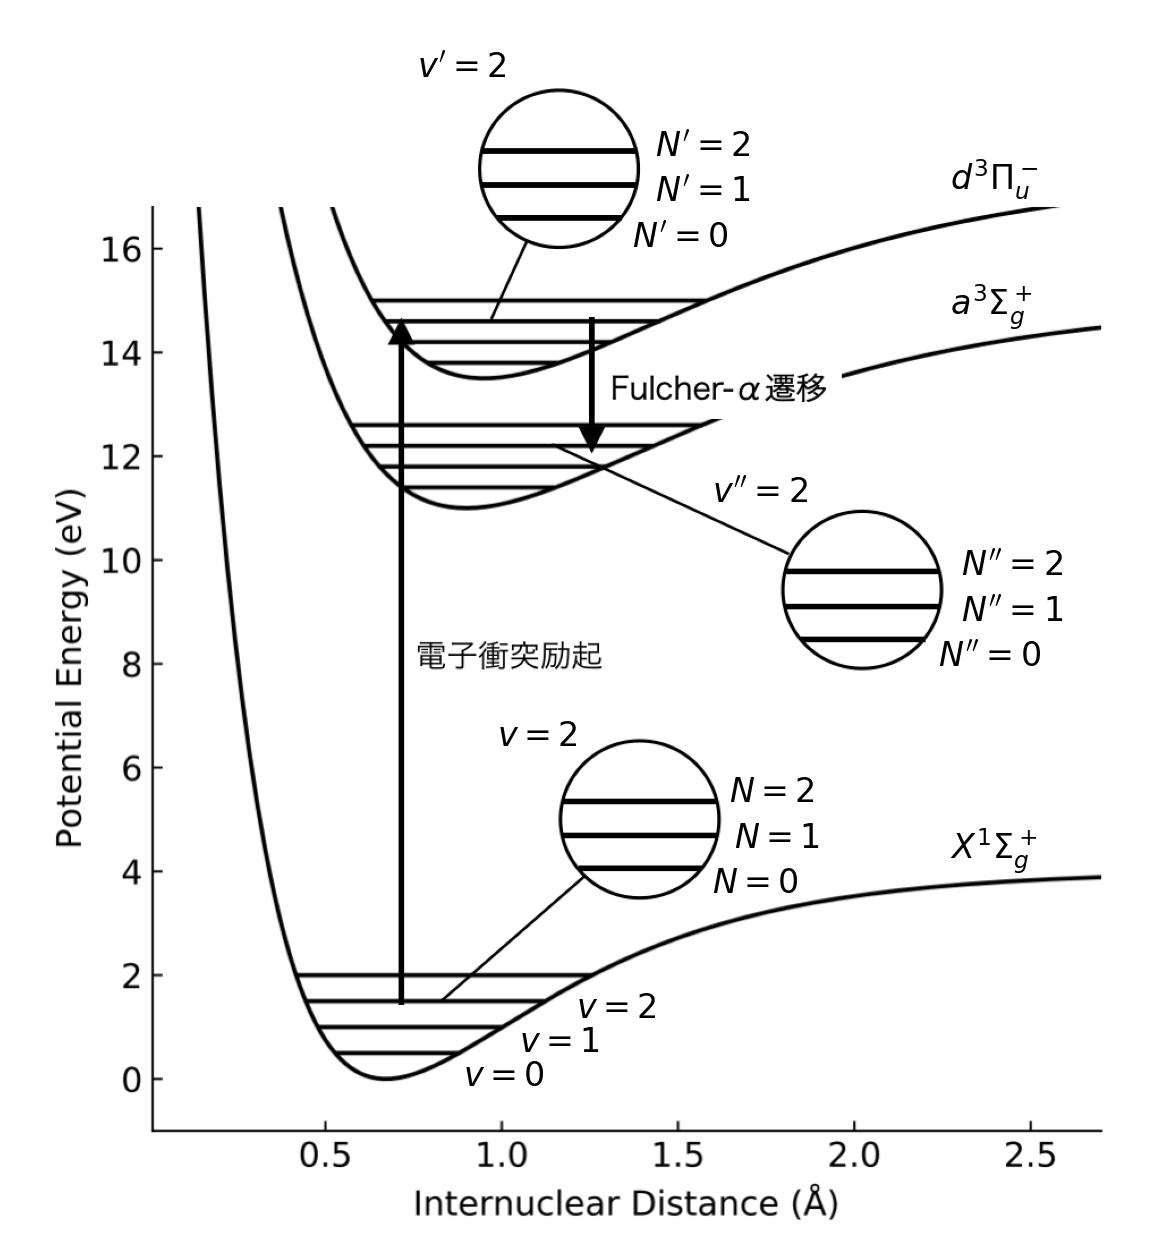
\includegraphics[width=15cm]{pictures/energy-level.png}
    \caption{$H_2$のポテンシャル曲線}
    \label{fig:energy-level}
\end{figure}

\begin{figure}
    \centering
    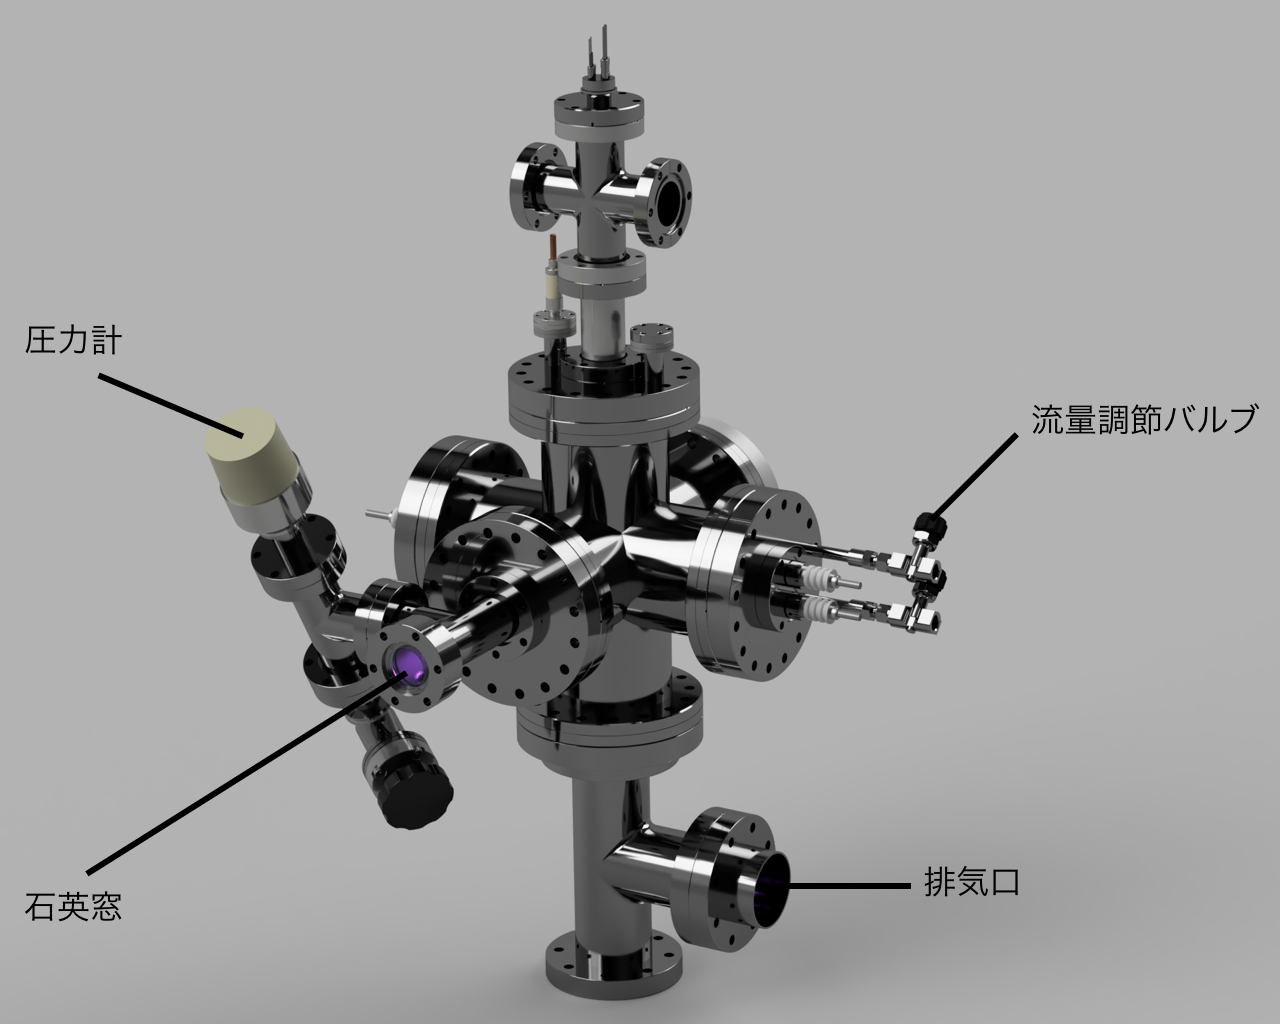
\includegraphics[width=15cm]{pictures/chamber-picture.png}
    \caption{プラズマチャンバの外観}
    \label{fig:chamber-picture}
\end{figure}

\begin{figure}
    \centering
    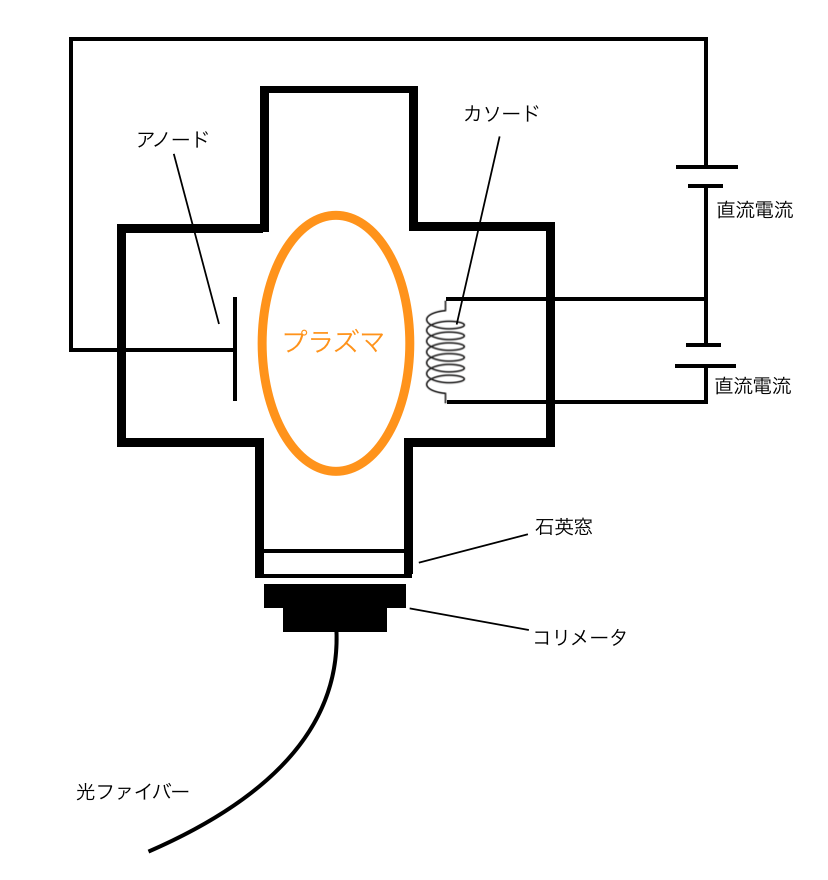
\includegraphics[width=15cm]{pictures/chamber-simple.png}
    \caption{プラズマチャンバの構造の簡略図}
    \label{fig:chamber-simple}
\end{figure}

\begin{figure}
    \centering
    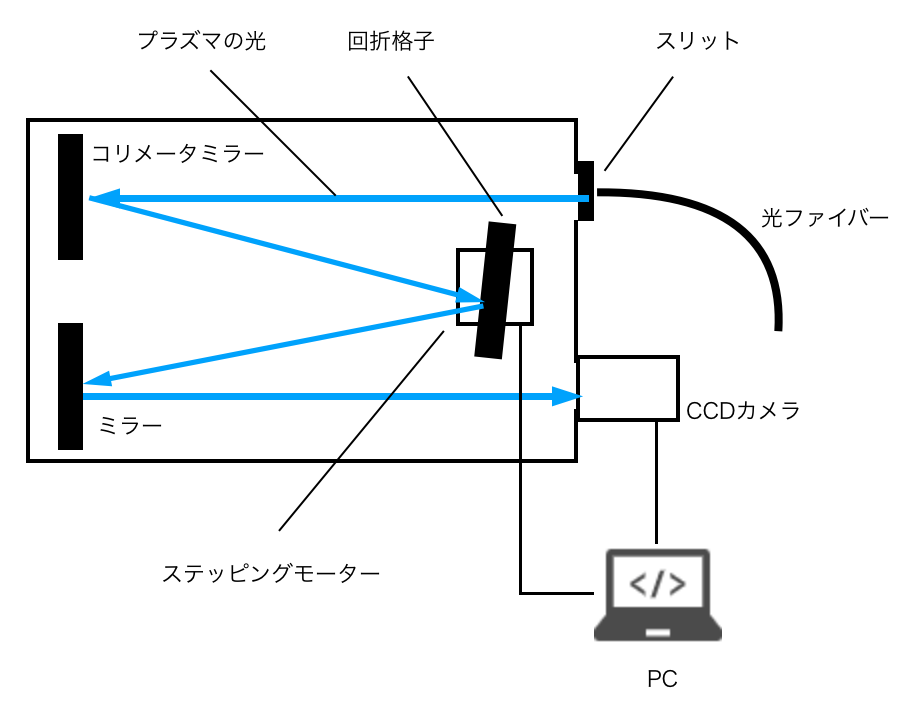
\includegraphics[width=15cm]{pictures/spectrometer-picture.png}
    \caption{分光器の概略図}
    \label{fig:spectrometer-picture}
\end{figure}

\begin{figure}
    \centering
    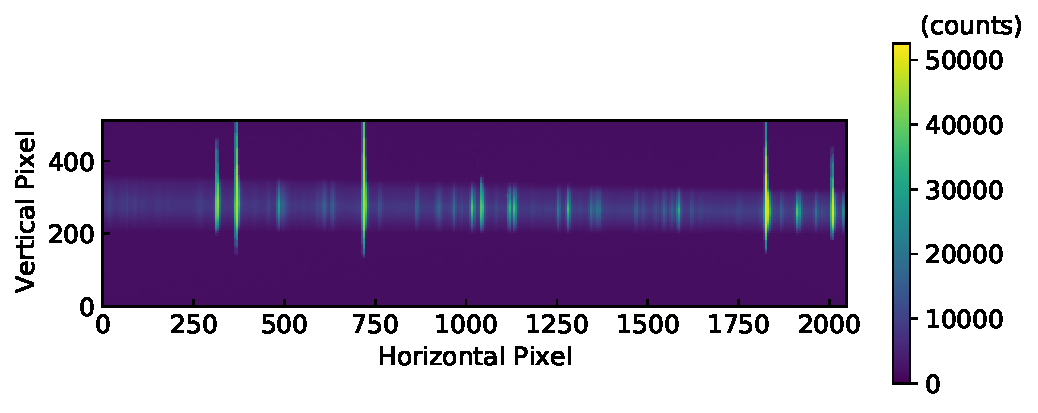
\includegraphics[width=15cm]{pictures/picture-example.pdf}
    \caption{CCDカメラで撮影した画像の例}
    \label{fig:picture-example}
\end{figure}

\begin{figure}
    \centering
    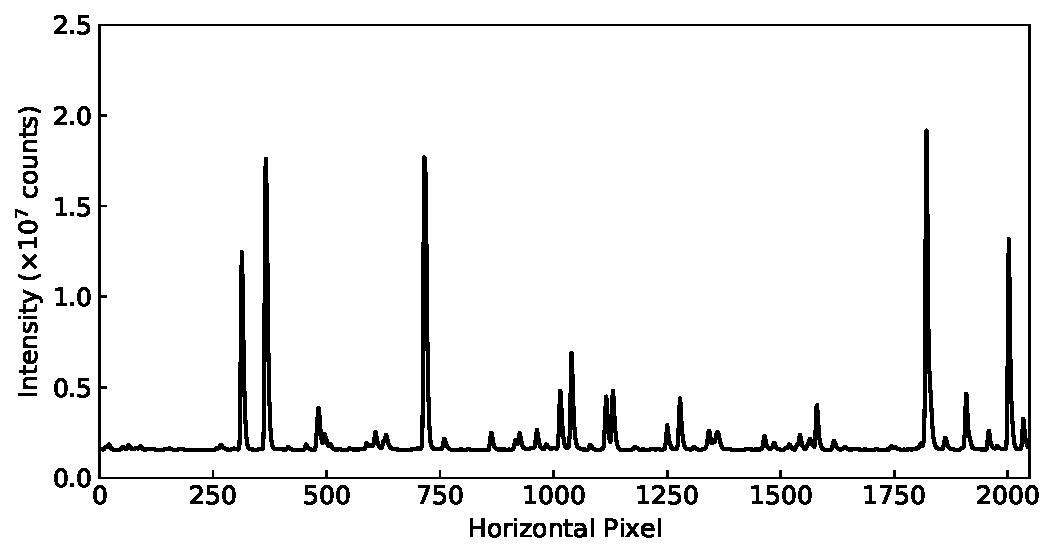
\includegraphics[width=15cm]{pictures/spectrum-example.pdf}
    \caption{画像のピクセル値を縦に合計したグラフの例}
    \label{fig:spectrum-example}
\end{figure}

\begin{figure}
    \centering
    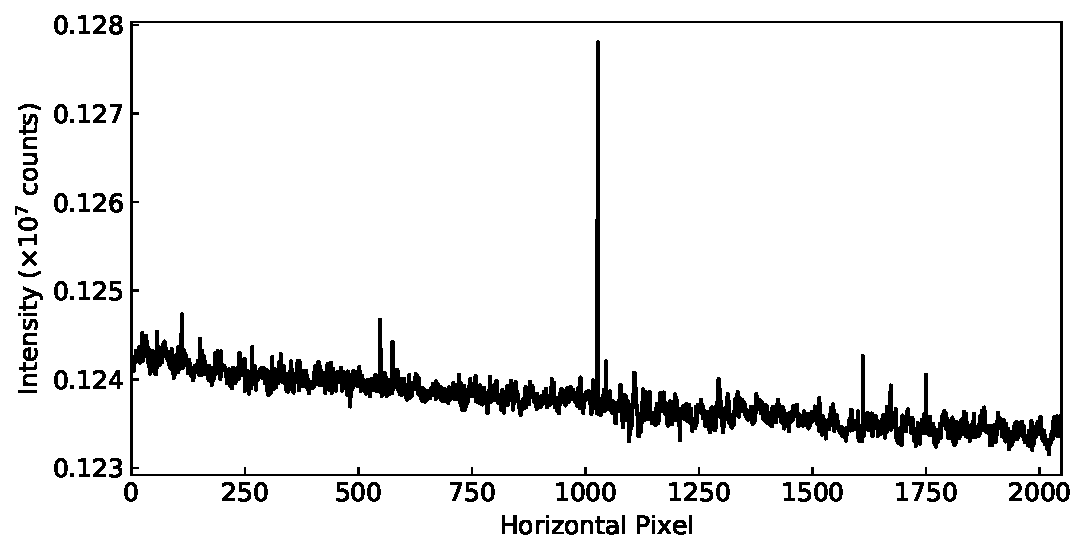
\includegraphics[width=15cm]{pictures/back-spectrum-example.pdf}
    \caption{バックグラウンドデータの例}
    \label{fig:back-spectrum-example}
\end{figure}

\begin{figure}
    \centering
    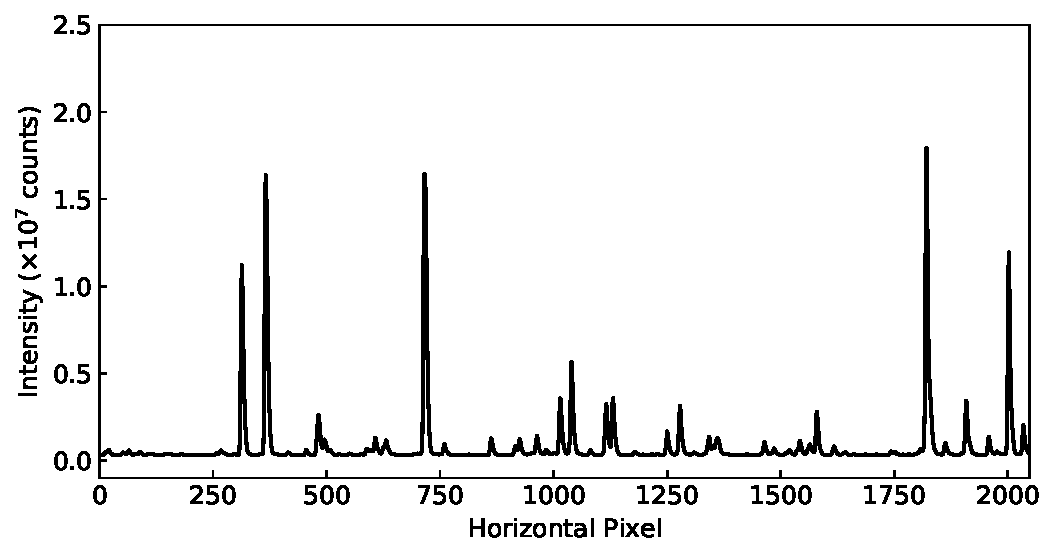
\includegraphics[width=15cm]{pictures/true-spectrum-example.pdf}
    \caption{バックグラウンドを除いたスペクトルの例}
    \label{fig:true-spectrum-example}
\end{figure}

\begin{figure}
    \centering
    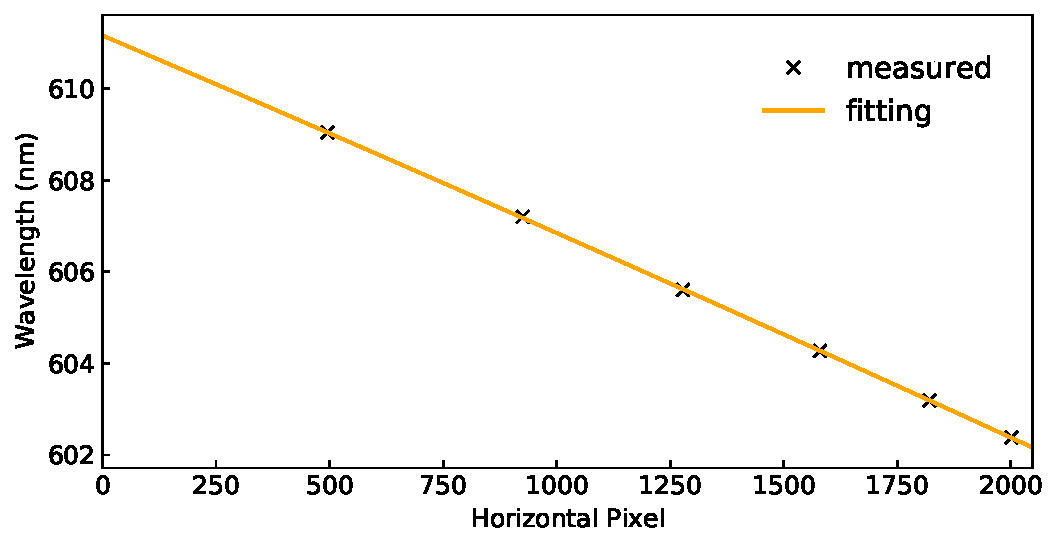
\includegraphics[width=15cm]{pictures/pixel-to-wavelength.pdf}
    \caption{ピクセルと波長の関係の例}
    \label{fig:pixel-to-wavelength}
\end{figure}

\begin{figure}
    \centering
    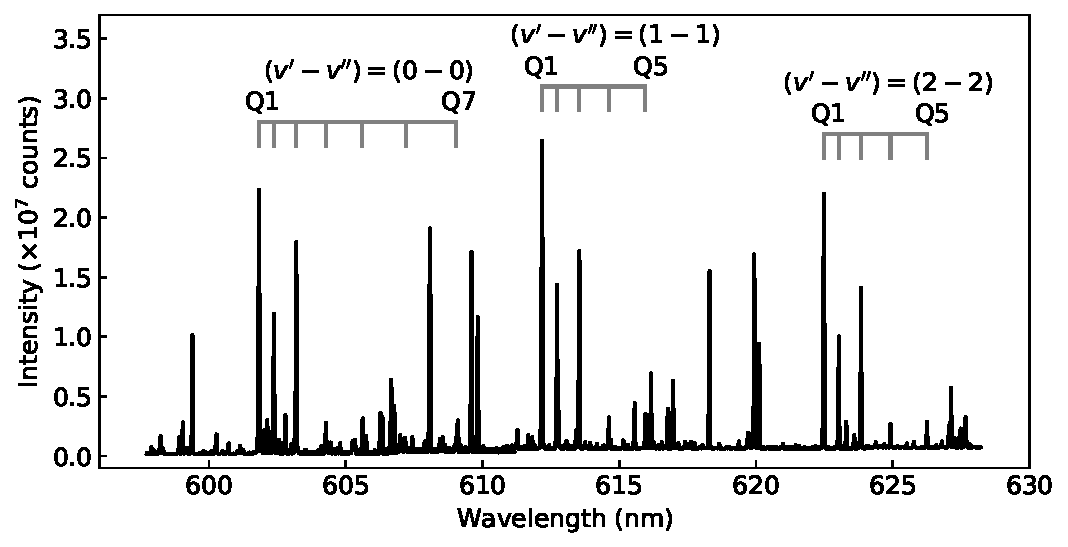
\includegraphics[width=15cm]{pictures/all-spectrum.pdf}
    \caption{Fulcher-α帯Q枝発光スペクトル}
    \label{fig:all-spectrum}
\end{figure}

\begin{figure}
    \centering
    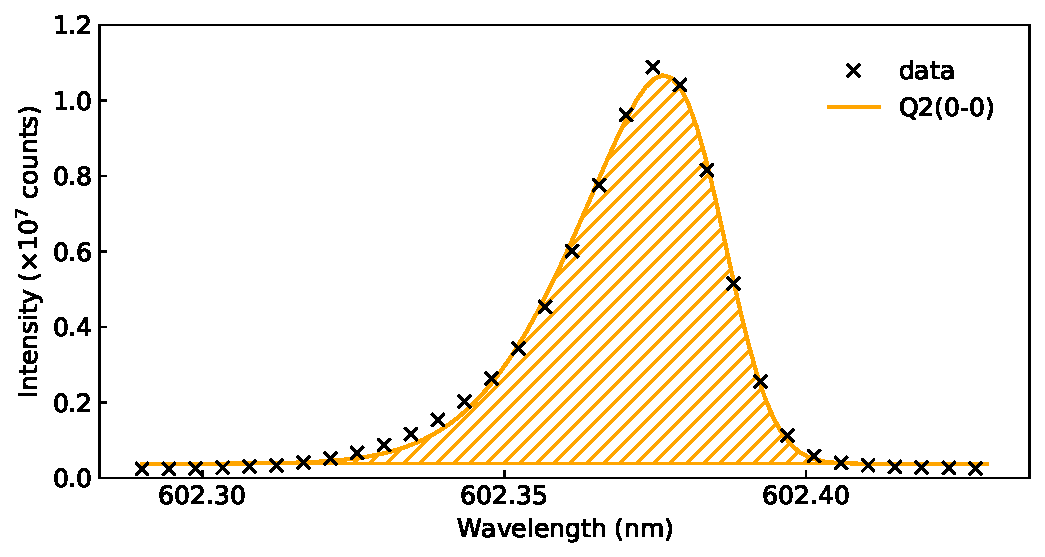
\includegraphics[width=15cm]{pictures/skewed-gaussian-fitting-00_Q2.pdf}
    \caption{歪正規分布関数によるフィッティングの例}
    \label{fig:voigt-fitting-1}
\end{figure}

\begin{figure}
    \centering
    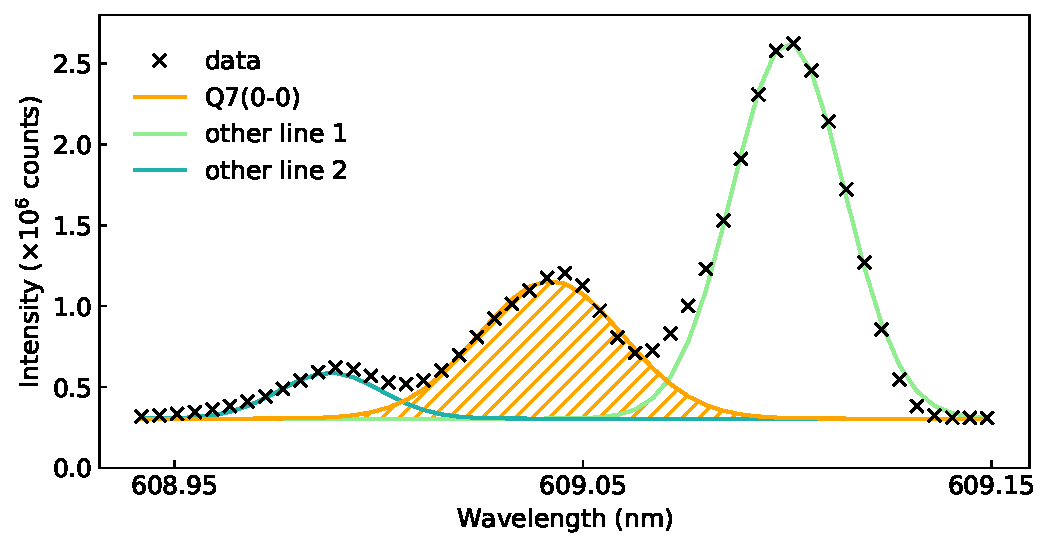
\includegraphics[width=15cm]{pictures/skewed-gaussian-fitting-00_Q7.pdf}
    \caption{歪正規分布関数フィッティングによる分離の例}
    \label{fig:voigt-fitting-2}
\end{figure}

\begin{figure}
    \centering
    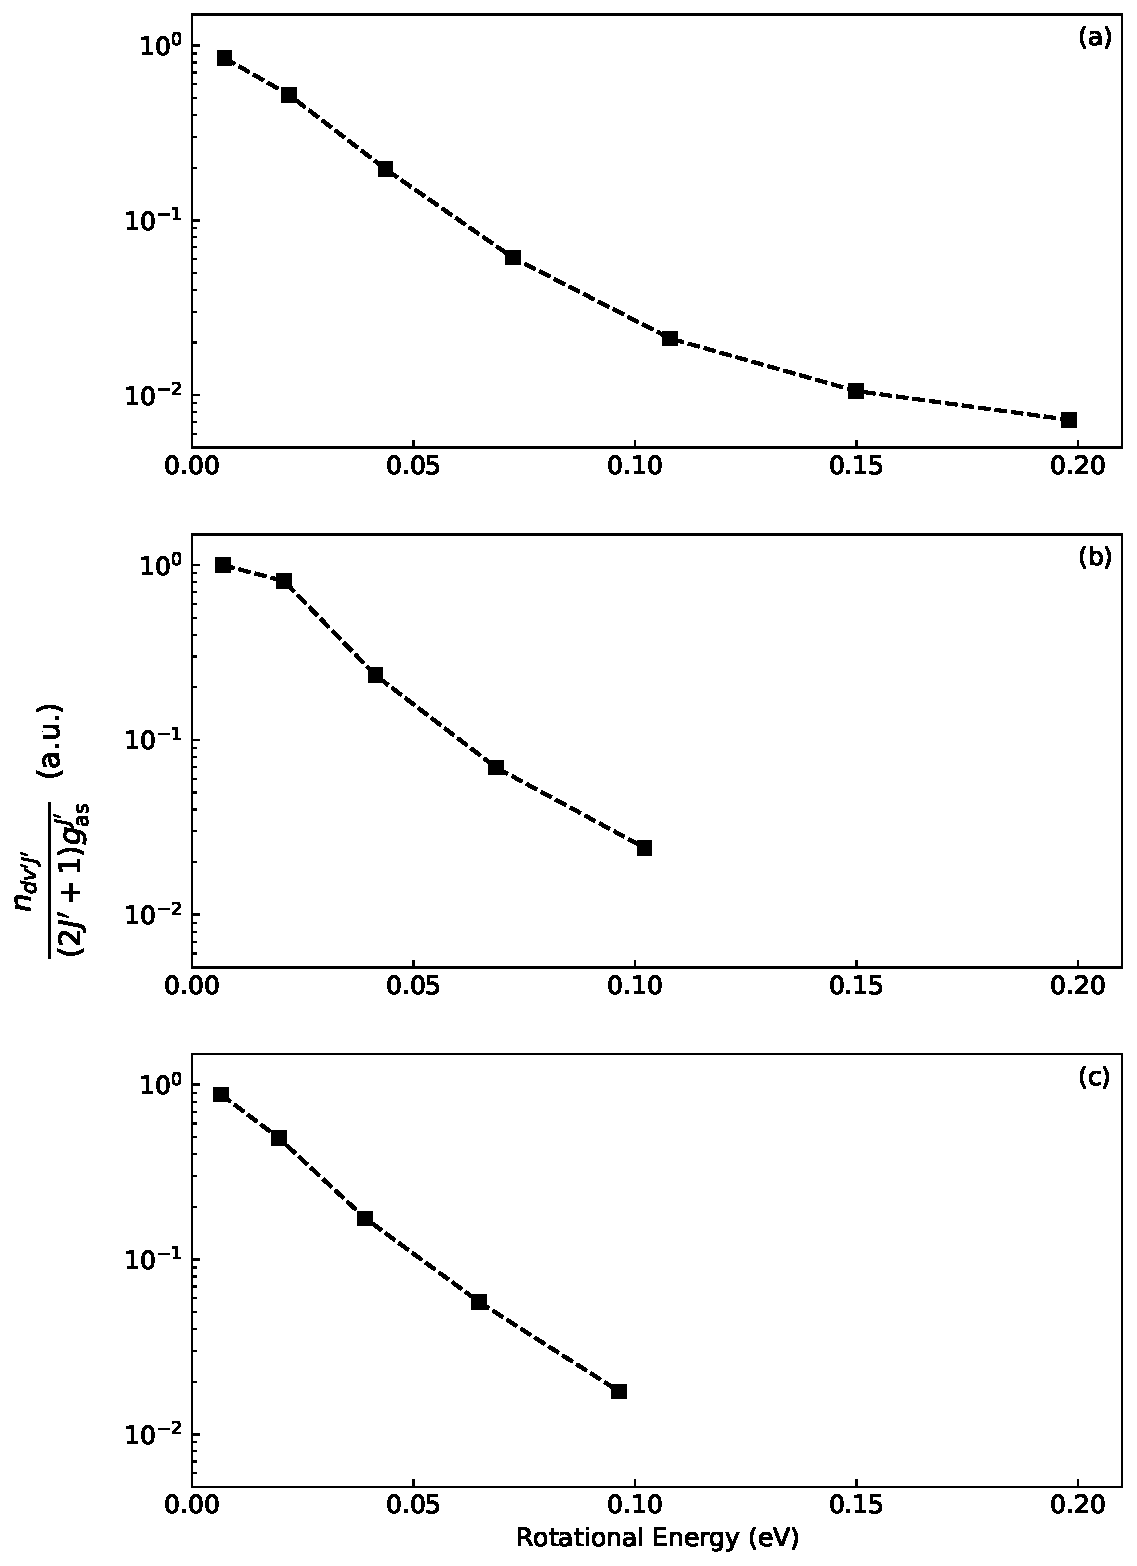
\includegraphics[width=15cm]{pictures/upper-boltzmann-plot.pdf}
    \caption{上準位占有数のボルツマンプロット}
    \label{fig:upper-boltzmann-plot}
\end{figure}

\begin{figure}
    \centering
    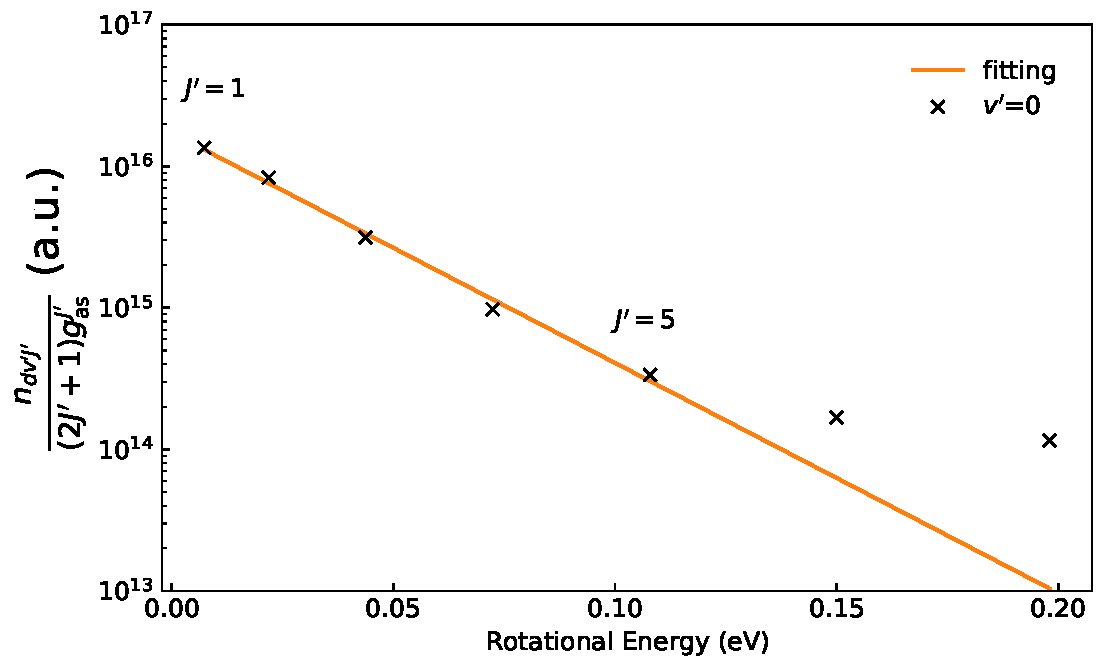
\includegraphics[width=15cm]{pictures/upper-fitting-0.pdf}
    \caption{発光上準位回転温度のフィッティング($v'=0$)}
    \label{fig:upper-fitting-0}
\end{figure}

\begin{figure}
    \centering
    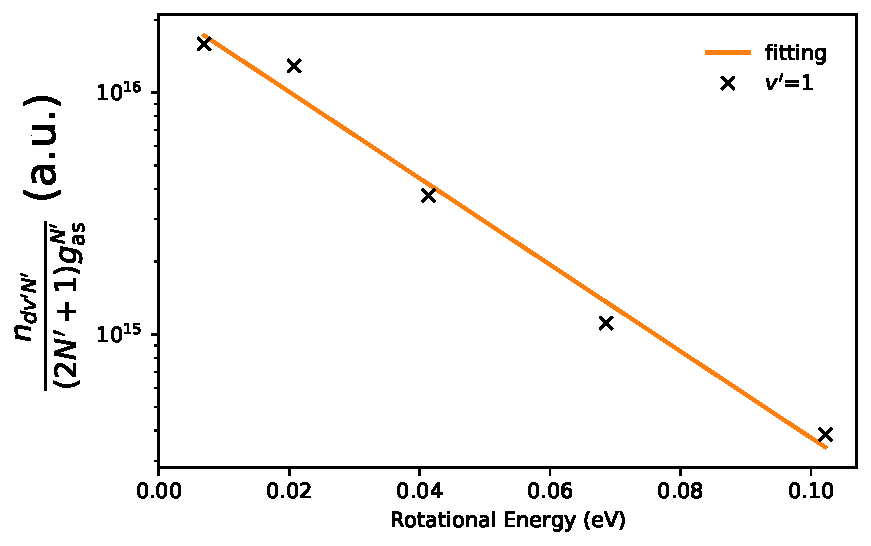
\includegraphics[width=15cm]{pictures/upper-fitting-1.pdf}
    \caption{発光上準位回転温度のフィッティング($v'=1$)}
    \label{fig:upper-fitting-1}
\end{figure}

\begin{figure}
    \centering
    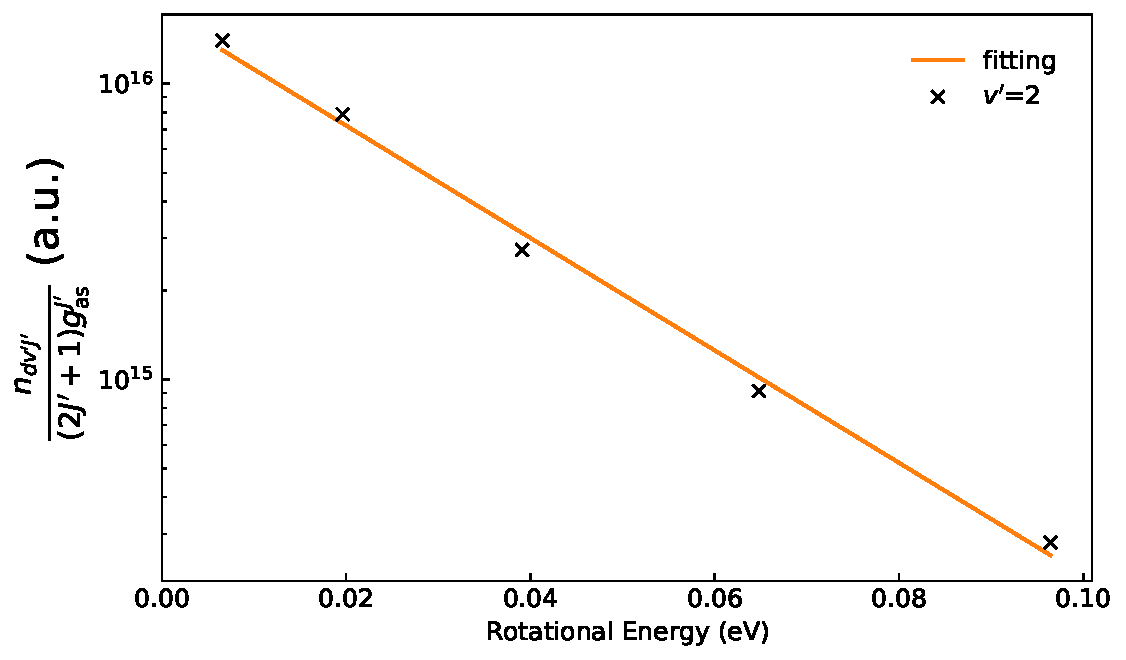
\includegraphics[width=15cm]{pictures/upper-fitting-2.pdf}
    \caption{発光上準位回転温度のフィッティング($v'=2$)}
    \label{fig:upper-fitting-2}
\end{figure}

\begin{figure}
    \centering
    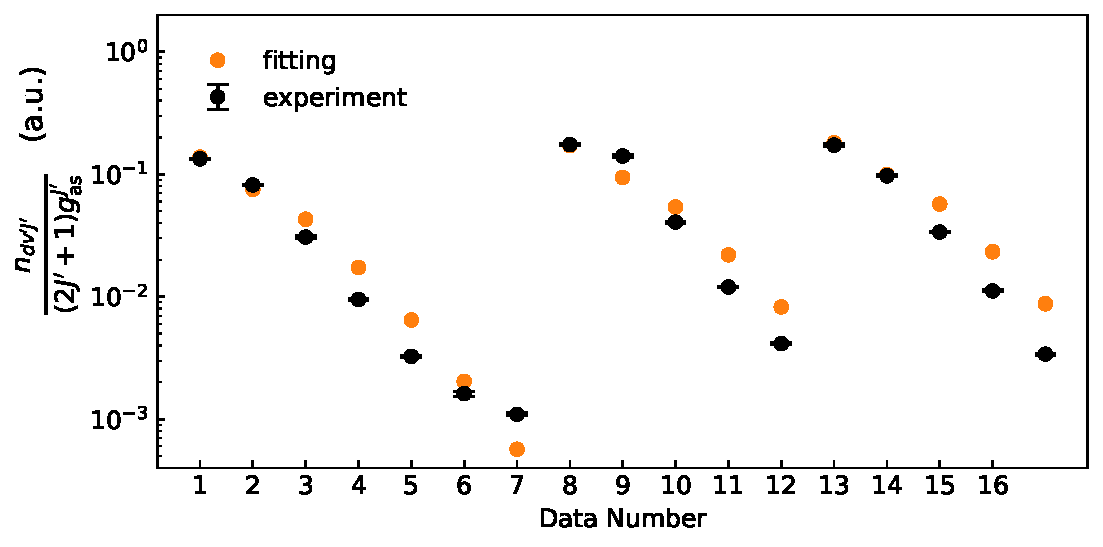
\includegraphics[width=15cm]{pictures/fitting-result.pdf}
    \caption{基底準位振動温度のフィッティング結果}
    \label{fig:fitting-result}
\end{figure}

\begin{figure}
    \centering
    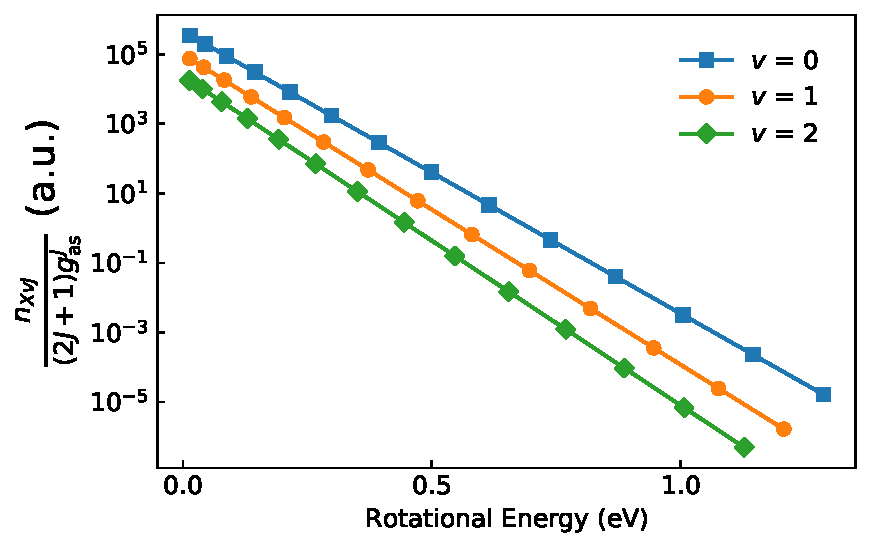
\includegraphics[width=15cm]{pictures/ground-state-n.pdf}
    \caption{基底準位の占有数分布}
    \label{fig:ground-state-n}
\end{figure}

\begin{figure}
    \centering
    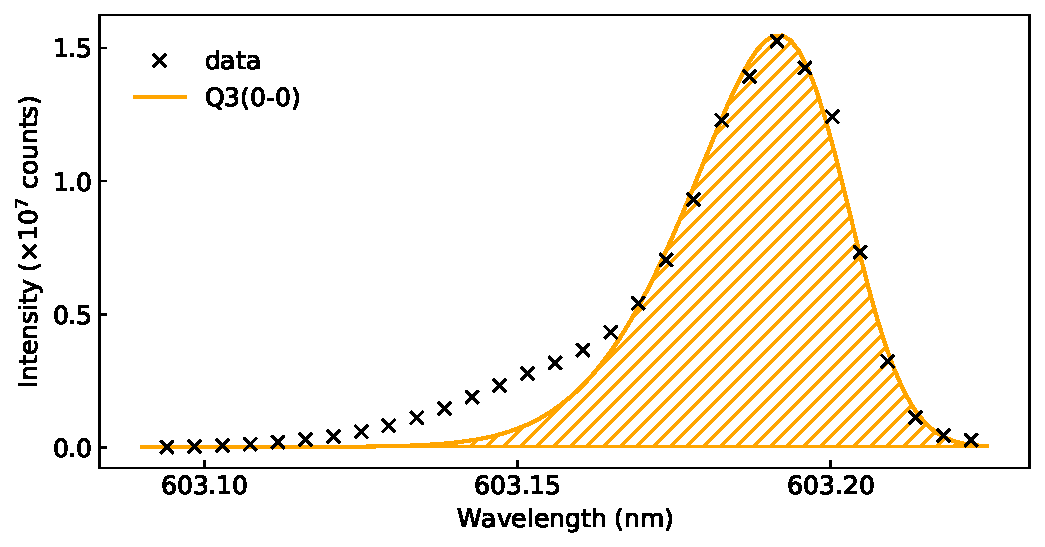
\includegraphics[width=15cm]{pictures/skewed-gaussian-fitting-00_Q3.pdf}
    \caption{Q3(0-0)スペクトル}
    \label{fig:voigt-fitting-3}
\end{figure}

\begin{figure}
    \centering
    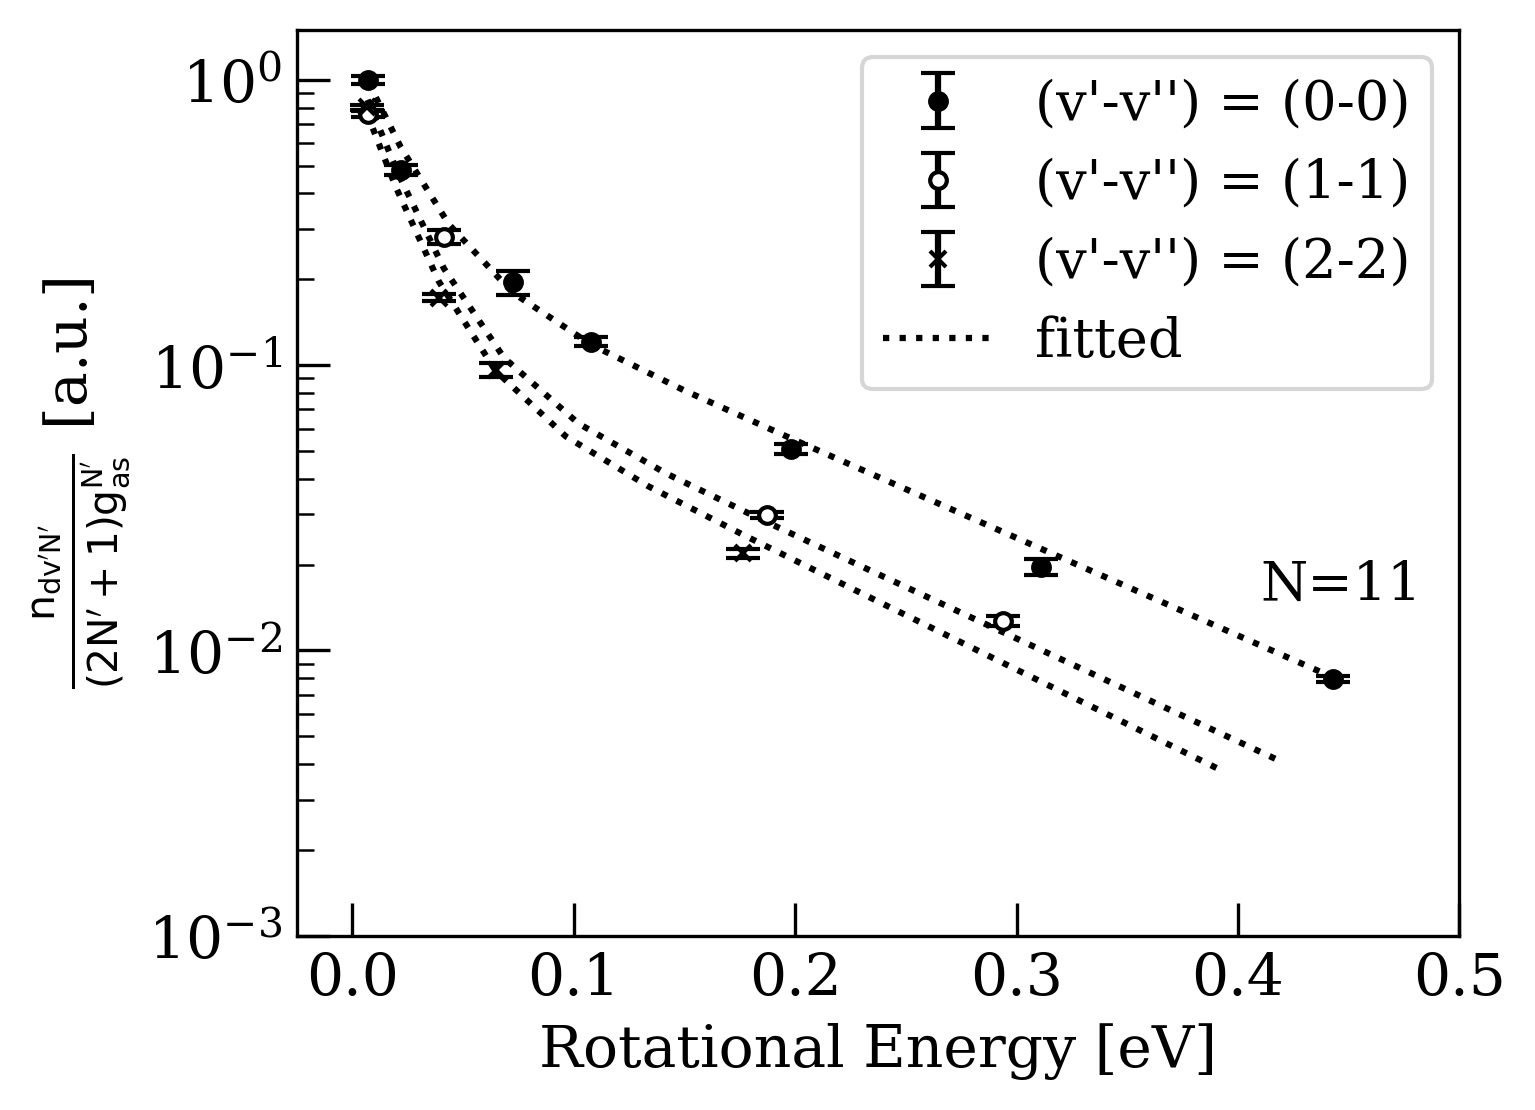
\includegraphics[width=15cm]{pictures/ishihara-upper-boltzmann.png}
    \caption{LHDでの上準位占有数のボルツマンプロット}
    \label{fig:ishihara-upper-boltzmann}
\end{figure}
